\documentclass[12pt, letterpaper]{article}
\usepackage{graphicx}
\usepackage{subcaption}
\usepackage{float}
\usepackage[spanish,es-tabla]{babel}
\graphicspath{{img/}}


\begin{document}

\begin{center}
    ''Año del Fortalecimiento de la Soberania Nacional''
    \vspace{5mm}
    \begin{figure}[h]
        \centering
        
\includegraphics[width=4cm,height=4cm]{UNMSM}
    \end{figure}

    \textbf{Universidad Nacional Mayor de San marcos} \\
    (Universidad del Perú,DECANA DE AMERICA)\\
    \vspace{5mm}
    FACULTAD DE INGENIERIA DE SISTEMAS E INFORMATICA
    Escuela Profesional de Ingenieria de Software
    \begin{figure}[h]
        \centering   
        
\includegraphics[width=2cm,height=2cm]{FISI}   
    \end{figure}

\textbf{\underline{Primera EC: Laboratorio Open MP}}

    \begin{flushleft}
    \textbf{Curso:}Programacion Paralela y Concurrente\\
    \vspace{2mm}
    \textbf{Profesor:} Edson Ticona Zegarra\\
    \vspace{2mm}
    \textbf{Integrantes:} 
    \begin{itemize}
        \item Pichilingue Pimentel, Nathaly Nicole\hspace{1cm} 19200247
        \item Torre Arteaga, Alexander\hspace{3.2cm}19200246
        \item Ricse Perez, Anthony Elias\hspace{3cm}19200276
    \end{itemize}
    \end{flushleft}

    Ciudad Universitaria 2022
 
\end{center}

\vspace{10mm}
\begin{flushleft}
    \textbf{Entorno de pruebas:}
    \begin{itemize}
        \item Procesador: AMD Ryzen 5 3500U with Radeon Vega Mobile Gfx  2.10 GHz
        \item Memoria RAM: 16 GB
        \item Número de procesadores: 8
        \item Sistema Operativo: Windows 10 Home
        \item IDE para pruebas: Dev C++
        \item IDE de desarrollo: Visual Studio Code
    \end{itemize}
    \textbf{Versión Secuencial}\\
    Ejecutamos la versión secuencial 10 veces para, en base a ello, poder analizar el tiempo de ejecución en gráficas.
    \begin{table}[h]
        \begin{center}
            \begin{tabular}{| c | c |}
                \hline
                Vez & Cantidad \\ \hline
                1 & 0.0362661 \\\hline
                2 & 0.0362704 \\\hline
                3 & 0.0362803 \\ \hline
                4 & 0.0367448 \\ \hline
                5 & 0.0357731 \\ \hline
                6 & 0.0360422 \\ \hline
                7 & 0.0176593 \\ \hline
                8 & 0.0388498 \\ \hline
                9 & 0.0357934 \\ \hline
                10 & 0.0353939 \\ \hline
            \end{tabular}
            \caption{Tiempos de ejecución versión secuencial}
            \label{tab:sec}
        \end{center}
    \end{table}
\end{flushleft}
\begin{flushleft}
    \begin{figure}[H]
        \begin{subfigure}{0.49\textwidth}
            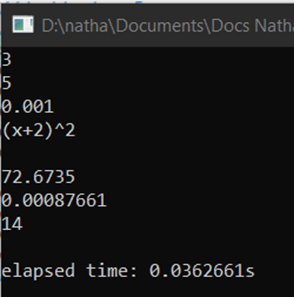
\includegraphics[width=1\linewidth, height=6cm]{Imagen1} 
        \end{subfigure}
        \begin{subfigure}{0.49\textwidth}
            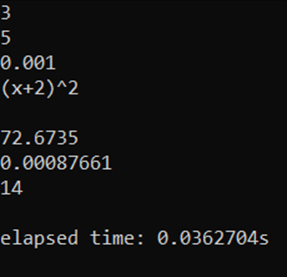
\includegraphics[width=1\linewidth, height=6cm]{Imagen2}
        \end{subfigure}
        \begin{subfigure}{0.49\textwidth}
            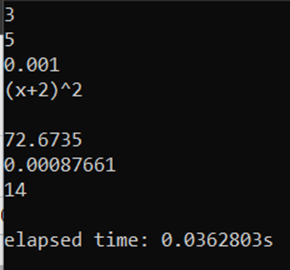
\includegraphics[width=1\linewidth, height=6cm]{Imagen3}
        \end{subfigure}
        \begin{subfigure}{0.49\textwidth}
            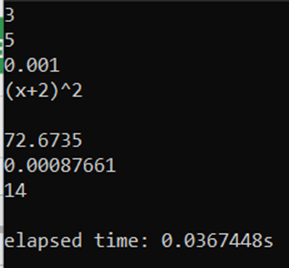
\includegraphics[width=1\linewidth, height=6cm]{Imagen4}
        \end{subfigure}
        \begin{subfigure}{0.49\textwidth}
            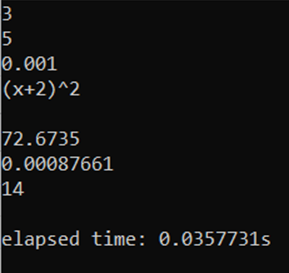
\includegraphics[width=1\linewidth, height=6cm]{Imagen5}
        \end{subfigure}
        \begin{subfigure}{0.49\textwidth}
            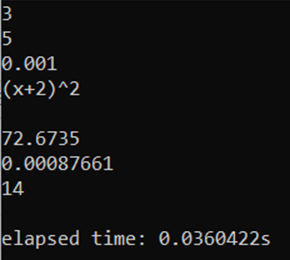
\includegraphics[width=1\linewidth, height=6cm]{Imagen6}
        \end{subfigure}
        \caption{Ejecucion 1 a 6 en orden de izquierda a derecha}
    \end{figure}
    \begin{figure}[H]
        \begin{subfigure}{0.49\textwidth}
            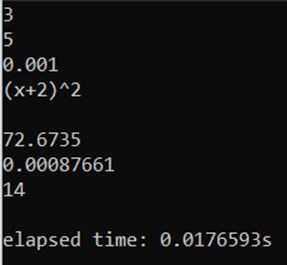
\includegraphics[width=1\linewidth, height=6cm]{Imagen7} 
        \end{subfigure}
        \begin{subfigure}{0.49\textwidth}
            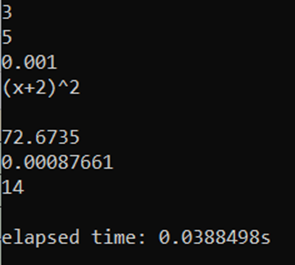
\includegraphics[width=1\linewidth, height=6cm]{Imagen8}
        \end{subfigure}
        \begin{subfigure}{0.49\textwidth}
            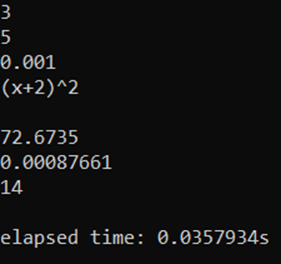
\includegraphics[width=1\linewidth, height=6cm]{Imagen9}
        \end{subfigure}
        \begin{subfigure}{0.49\textwidth}
            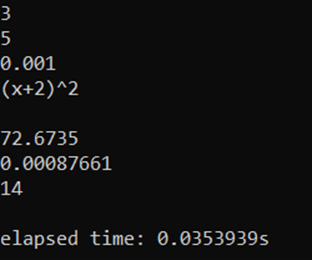
\includegraphics[width=1\linewidth, height=6cm]{Imagen10}
        \end{subfigure}
        \caption{Ejecucion 7 a 10 en orden de izquierda a derecha}
    \end{figure}
    
\end{flushleft}

\begin{flushleft}
    Y en gráfico de dispersión obtenemos el siguiente (Realizado con Python en Google Colab):

    \begin{figure}[H]
        \begin{flushleft}
            Y en gráfico de dispersión obtenemos el siguiente (Realizado con Python en Google Colab):
        \end{flushleft}
        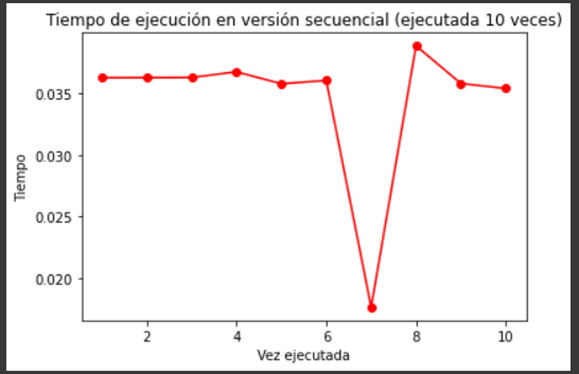
\includegraphics[width=1\linewidth, height=6cm]{Imagen11} 
        \caption{Tiempo de ejecución en version secuencial (ejecutada 10 veces)}
    \end{figure}
        Podemos observar que el tiempo de ejecución es en promedio 0.036 segundos, teniendo un valor divergente en la 7ma ejecución del programa donde se obtuvo un tiempo de 0.017 segundos.
\end{flushleft}
\textbf{Versión Paralela}\\
Ejecutamos la versión paralela 10 veces para, en base a ello, poder analizar el tiempo de ejecución en gráficas.
\begin{table}[h]
    \begin{center}
        \begin{tabular}{| c | c |}
            \hline
            Vez & Cantidad \\ \hline
            1 & 0.0144939 \\\hline
            2 & 0.0142298 \\\hline
            3 & 0.0143356 \\ \hline
            4 & 0.0149603 \\ \hline
            5 & 0.0154302 \\ \hline
            6 & 0.0146521 \\ \hline
            7 & 0.0140904 \\ \hline
            8 & 0.0161136 \\ \hline
            9 & 0.0144786 \\ \hline
            10 & 0.0142954 \\ \hline
        \end{tabular}
        \caption{Tiempos de ejecución versión paralela}
        \label{tab:par}
    \end{center}
\end{table}


\begin{figure}[H]
    \begin{subfigure}{0.49\textwidth}
        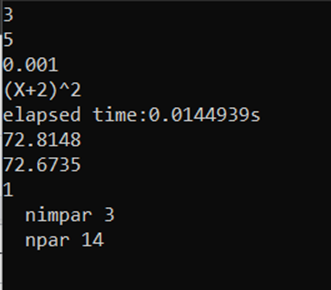
\includegraphics[width=1\linewidth, height=6cm]{Imagen12} 
    \end{subfigure}
    \begin{subfigure}{0.49\textwidth}
        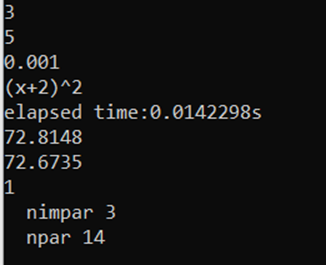
\includegraphics[width=1\linewidth, height=6cm]{Imagen13}
    \end{subfigure}
    \begin{subfigure}{0.49\textwidth}
        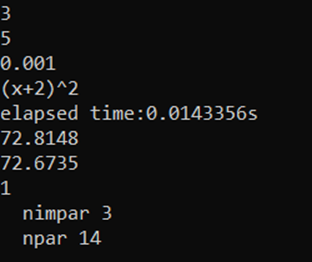
\includegraphics[width=1\linewidth, height=6cm]{Imagen14}
    \end{subfigure}
    \begin{subfigure}{0.49\textwidth}
        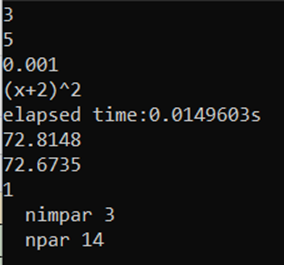
\includegraphics[width=1\linewidth, height=6cm]{Imagen15}
    \end{subfigure}

    \caption{Ejecucion 12 a 15 en orden de izquierda a derecha}
\end{figure}
\begin{figure}[H]
    \begin{subfigure}{0.49\textwidth}
        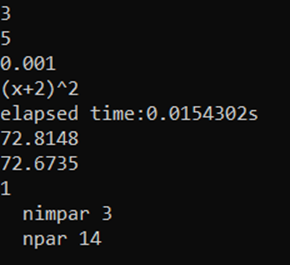
\includegraphics[width=1\linewidth, height=6cm]{Imagen16}
    \end{subfigure}
    \begin{subfigure}{0.49\textwidth}
        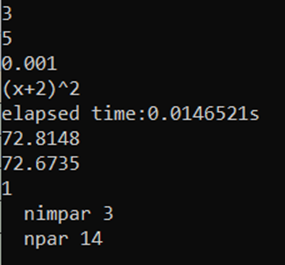
\includegraphics[width=1\linewidth, height=6cm]{Imagen17}
    \end{subfigure}
    \begin{subfigure}{0.49\textwidth}
        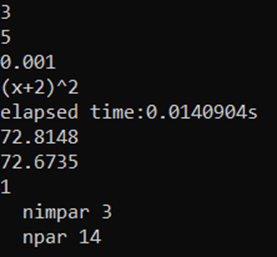
\includegraphics[width=1\linewidth, height=6cm]{Imagen18} 
    \end{subfigure}
    \begin{subfigure}{0.49\textwidth}
        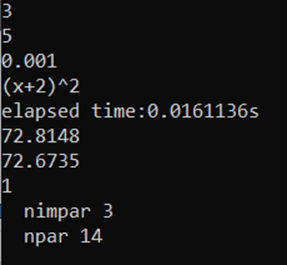
\includegraphics[width=1\linewidth, height=6cm]{Imagen19}
    \end{subfigure}
    \begin{subfigure}{0.49\textwidth}
        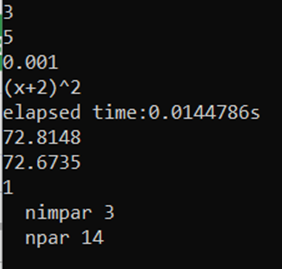
\includegraphics[width=1\linewidth, height=6cm]{Imagen20}
    \end{subfigure}
    \begin{subfigure}{0.49\textwidth}
        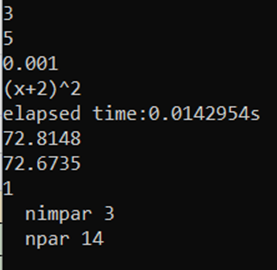
\includegraphics[width=1\linewidth, height=6cm]{Imagen21}
    \end{subfigure}
    \caption{Ejecucion 16 a 21 en orden de izquierda a derecha}
\end{figure}

\begin{flushleft}
    Y en gráfico de dispersión obtenemos el siguiente (Realizado con Python en Google Colab):    
    \begin{figure}[H]
        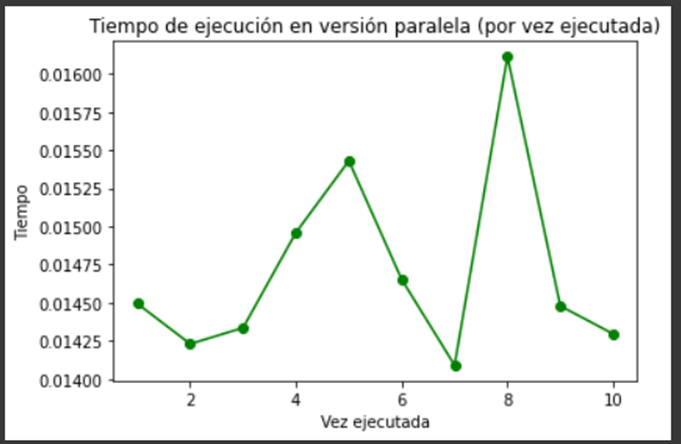
\includegraphics[width=1\linewidth, height=6cm]{Imagen23} 
        \caption{Tiempo de ejecución en version paralela}
    \end{figure}
    Podemos observar que el tiempo de ejecución es en promedio 0.014 segundos, teniendo dos valores divergentes en la 5ta y 8va vez de ejecución, de 0.015 y 0.018 segundos respectivamente.
    \begin{figure}[H]
        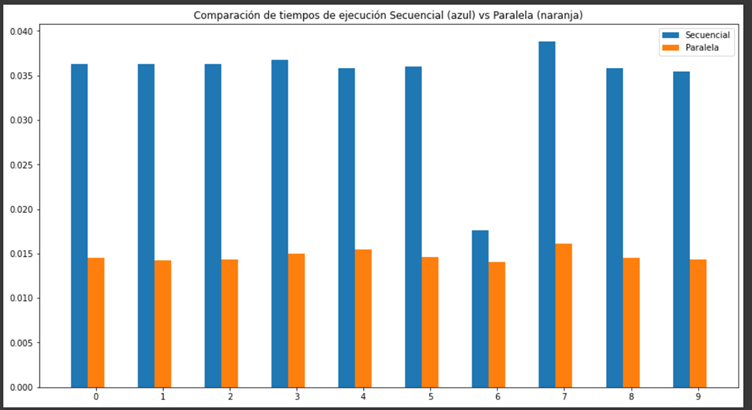
\includegraphics[width=1\linewidth, height=6cm]{Imagen24}
        \caption{Comparacion de tiempos algoritmos secuencial vs paralelo}
    \end{figure}
    \begin{figure}[H]
        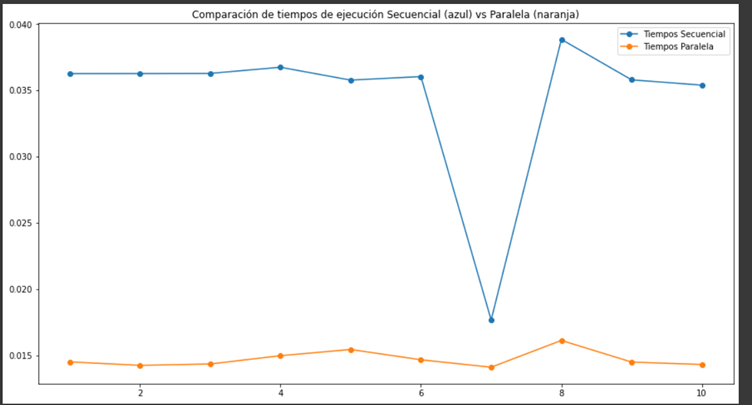
\includegraphics[width=1\linewidth, height=6cm]{Imagen25}
        \caption{Comparacion de tiempos algoritmo secuencial vs paralelo}
    \end{figure}
    Se realizó un gráfico de barras comparando los tiempos de ejecución entre la versión Secuencial y la versión Paralela, donde se encontró por amplio margen que la versión paralela tiene un tiempo de ejecución mucho menor que la versión secuencial, es decir, es más rápido al realizar la ejecución del programa, esto debido a que, en el método del trapecio, la versión paralela divide en distintas particiones (como pares e impares) y ejecuta esas varias particiones en simultáneo, no debe esperar a la anterior, por lo tanto, obtiene la solución mucho más rápido.
\end{flushleft}


\end{document}